\documentclass[10pt,twocolumn,letterpaper]{article}
%% Welcome to Overleaf!
%% If this is your first time using LaTeX, it might be worth going through this brief presentation:
%% https://www.overleaf.com/latex/learn/free-online-introduction-to-latex-part-1

%% Researchers have been using LaTeX for decades to typeset their papers, producing beautiful, crisp documents in the process. By learning LaTeX, you are effectively following in their footsteps, and learning a highly valuable skill!

%% The \usepackage commands below can be thought of as analogous to importing libraries into Python, for instance. We've pre-formatted this for you, so you can skip right ahead to the title below.

%% Language and font encodings
\usepackage[english]{babel}
\usepackage[utf8x]{inputenc}
\usepackage[T1]{fontenc}
\usepackage{amsmath}

%% Sets page size and margins
\usepackage[a4paper,top=3cm,bottom=2cm,left=3cm,right=3cm,marginparwidth=1.75cm]{geometry}

%% Useful packages
\usepackage{amsmath}
\usepackage{graphicx}
\usepackage[colorinlistoftodos]{todonotes}
\usepackage[colorlinks=true, allcolors=blue]{hyperref}
\usepackage{natbib}
\bibliographystyle{unsrt}
%% Title
\title{
		\usefont{OT1}{bch}{b}{n}
		\normalfont \normalsize \textsc{SPH 3U1} \\ [10pt]
		\huge Work and Energy Lab Report \\
}
\selectlanguage{english}
\usepackage{authblk}
\author[1]{Hanz Nathan Po}

\begin{document}
\maketitle

\section{Objective}
The objective of this lab is to apply the law of conservation of energy in a real world scenario, using equations regarding work and energy.

\section{Introduction}
Energy is defined as the capacity for doing work. With that in mind, this experiment explores the various forms of energy that take effect when a basketball is thrown from one person to another. For the purposes of this experiment, only gravitational potential energy and kinetic energy are taken into account. The effects of other forms of potential energy, and air resistance are negligible. Based on the law of conservation of energy, which states that energy cannot be created nor destroyed, only converted from one form to another, it is known that
\begin{equation}
    E_{T}={E_{T}}'
\end{equation}
where \({E}_{T}\) is the initial total energy of the object, and \({E}_{T}'\) is the final total energy of the object. As mentioned earlier, as only gravitational potential energy and kinetic energy are being considered, it can be said that

\begin{equation}
    E_{T}=E_{g}+E_{k}
\end{equation}

where \({E}_{g}\) is the gravitational potential energy, and \({E}_{k}\) is the kinetic energy. Typically, all energy values are measured in Joules (J), however, in this experiment, the mass of the ball is not taken into account Joules per Kilogram (J/kg) is used. Combining this equation with equation one, it can also be said that

\begin{equation}
    E_{g}+E_{k}={E_{g}}'+{E_{k}}'
\end{equation}

where \({E_{g}}'\) and \({E_{k}}'\) are the final gravitational potential energy and final kinetic energy, respectively. Gravitational potential energy can be calculated using the following equation

\begin{equation}
    E_{g}=mgh
\end{equation}

where \(m\) is the mass of the object in kg, \(g\) is the acceleration due to gravity (\(\simeq 9.8m/s^2\)), and \(h\) is the height of the object above the ground in m. Kinetic energy can be calculated using the following equation

\begin{equation}
    E_{k}=\frac{1}{2}mv^2
\end{equation}

where \(m\) is the mass of the object in kg and \(v\) is the total velocity of the object. In order to calculate the total velocity, we must use the Pythagorean theorem with the X and Y velocities. 

\begin{equation}
    v_{T}=\sqrt{{v_{x}}^2 + {v_{y}}^2}
\end{equation}

This \(v_{T}\) value will allow us to calculate the kinetic energy by using equation 5, as previously mentioned. 

\section{Materials \& Procedure}

In order to perform this experiment, a ball, a video recording device, and a few friends are necessary. To start, get two people to stand a reasonable distance apart from each other. Give the ball to one of the people. Get a third person to hold an object with a fixed length, preferably a metre. A fourth person is to record from a position in which all three other people are clearly visible. The person with the ball is to then throw it towards the other person, preferably allowing the ball to reach a significant height in the process. Using a software such as Logger Pro, plot data from the video and prepare it for analysis. Once imported into the software, calculate \(E_{g}\), \(E_{k}\), and \(E_{T}\). \(E_{T}\) is calculated by simply adding \(E_{k}\) and \(E_{T}\).

\begin{figure}
  \centering
  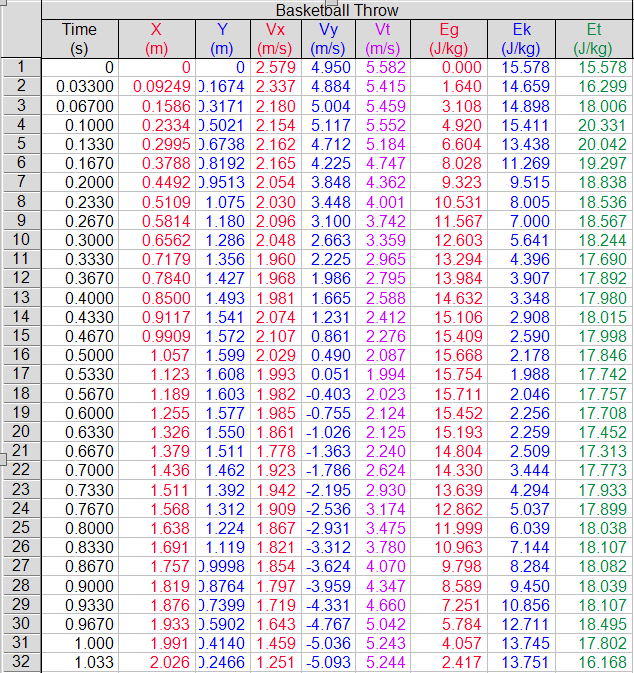
\includegraphics[width=0.5\textwidth]{figures/LoggerPro_voixZIMd34.png}
  \caption{Table of values generated from recording of projectile motion and energy calculations}
\end{figure}

\section{Analysis}

In figure 2, it is clear that the kinetic energy and gravitational potential energy values are both inversely proportional to each other. As the ball increases in altitude, its kinetic energy is transformed into gravitational potential energy, because its velocity is exchanged for altitude. 

At 0 seconds, the gravitational potential energy is zero, because as described in equation 4, if the height above the ground is zero, then the \(E_{g}\) must also be zero. 

\begin{align}
    \nonumber E_{g} = (1)(-9.8)(0) \\
    \nonumber E_{g} = 0 J/kg
\end{align}

As the ball increases in height, it also increases in \(E_{g}\), which means it will reach its maximum \(E_{g}\) at the maximum height. This can be calculated by solving for the time at which the height is at its maximum, then using the curve of best fit of the gravitational potential energy to calculate the \(E_{g}\) at that height. To find the time at apogee, we can find the derivative of the height function and set it equal to zero.

\begin{align}
    \nonumber h(\Delta t) = -5.590\Delta t^2+6.041\Delta t+0.031 \\
    \nonumber h'(\Delta t) = -11.18\Delta t+6.041 \\
    \nonumber -11.18\Delta t+6.041 = 0\\
    \nonumber -11.18\Delta t = -6.041\\
    \nonumber \Delta t \approx 0.54s
\end{align}

Now that we know the time at maximum height, we can solve for \(E_{g}\) as a function of time by using the curve of best fit found by Logger Pro.

\begin{align}
    \nonumber E_{g}(\Delta t) = -54.78\Delta t^2+59.21\Delta t-0.307 \\
    \nonumber E_{g}(0.54) = -54.78(0.54)^2+59.21(0.54)-0.307 \\
    \nonumber E_{g}(0.54) = 15.69 J/kg
\end{align}

For kinetic energy, because the ball has just started to fly through the air, the total velocity is at its highest value, meaning that the kinetic energy is also at its highest, as can be described by equation 5. By looking at the table of values, we can see that \(v_{T}\) is at its highest at 0 seconds (5.582 m/s). To find the kinetic energy at 0 seconds, we can use equation 5. 

\begin{equation}
    E_{k}=\frac{1}{2}(1)(5.582)^2
    E_{k}=15.58 J/kg
\end{equation}

As expected from the law of conservation of energy, the amount of kinetic energy at 0 seconds is very close to the amount of gravitational potential energy at the ball's maximum height, because most of the energy has been converted. A small amount of energy has been lost, likely due to other factors such as air resistance. As the ball falls from the maximum height, the energy is converted back again, as can be seen in figure 2, as well as the table of values in figure 1. This means that in a world without air resistence, the ball reaches its maximum kinetic energy again by the time it falls back down to a height of zero.

\begin{figure}
  \centering
  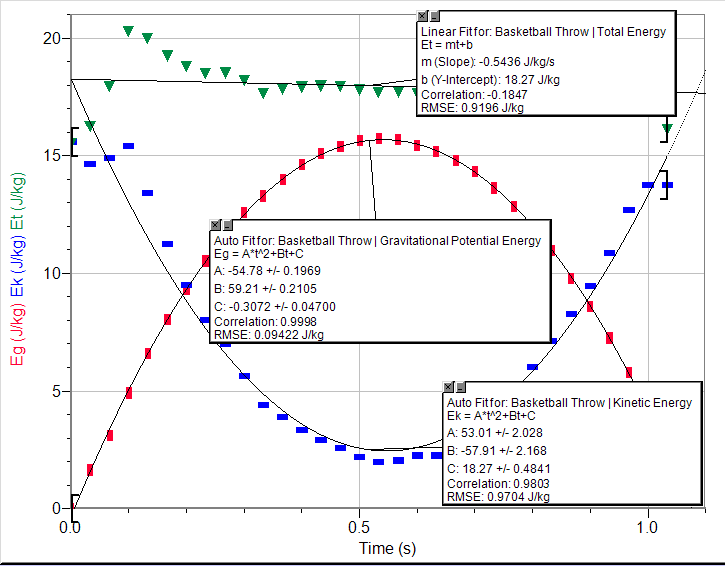
\includegraphics[width=0.5\textwidth]{figures/LoggerPro_pxxYVWhf00.png}
  \caption{Graph of the \(E_{g}\), \(E_{k}\), and \(E_{T}\) values over time. Values were calculated using formulas mentioned in the introduction, then linear and quadratic fits were plotted onto the graph.}
\end{figure}

\begin{figure}
  \centering
  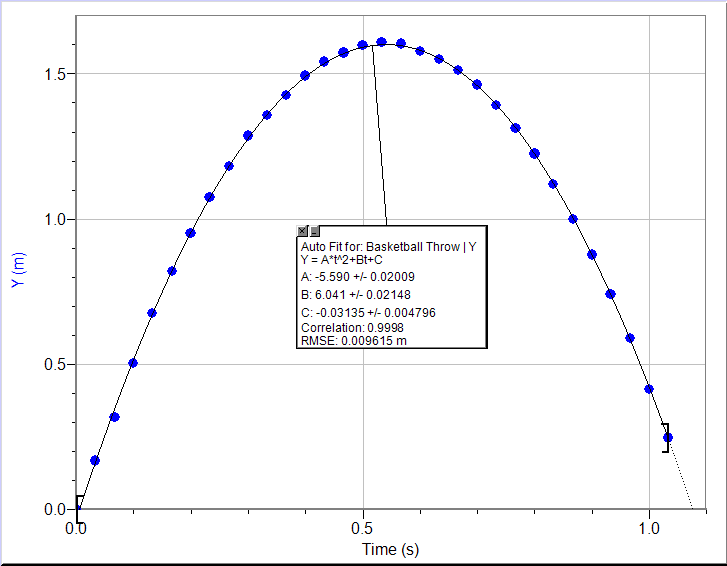
\includegraphics[width=0.5\textwidth]{figures/LoggerPro_twD1Xz5EFQ.png}
  \caption{Graph of the ball's height over time.}
\end{figure}

Therefore, the ball starts at its maximum kinetic energy, which is converted into gravitational potential energy over time, reaching its peak at the maximum height, then the energy is converted back into kinetic energy as the ball falls down. 

\section{Conclusion}
This experiment proved to be a very insightful way to look at how work and energy affect a projectile moving through the air. It was especially interesting to see that energy was mostly maintained throughout the projectile's flight, with energy simply being converted from one form to another, based on the height of the projectile. There were likely small sources of error during the plotting process, and from small sources of energy loss such as air resistance, which were not taken into account during the calculation process. 

\section{Discussion}
\subsection{Question One}
The slope of this line is -0.5426. This represents the energy that was not kinetic or gravitational potential energy in the system, in J/kg/s (the number of joules of energy in a 1 kg object in 1 second). 
\subsection{Question Two}
Question One does not contradict the law of conservation of energy. It is simply a reflection of the fact that there are factors such as air resistance which convert the energy into other forms which were not taken into account in the experiment. However, if this experiment were to be performed in a vacuum and plotted perfectly, there would be no slope on the line. 
\subsection{Question Three}
Due to the fact that mass was not taken into account, all calculations during the experiment were calculated in J/kg, or the amount of energy assuming an object with a mass of 1 kg. In order to account for differing masses, it is a matter of multiplying the energy per kilogram by the mass of the Ball. For example, if the kinetic energy of an object at 0 seconds is 15.58 J/kg, and the mass of the object is 20 kg, we can find the number of Joules by multiplying 15.58 by 20, giving us 311.6 J. 
\subsection{Question Four}
This can be done by subtracting the final total energy from the initial total energy, from the line of best fit. 

\begin{align}
    \nonumber E_{friction} = E_{Ti} - E_{Tf} \\
    \nonumber E_{friction} = 18.27 - 17.67 \\
    \nonumber E_{friction} = 0.596 J/kg
\end{align}

\end{document}